% ======================================================================
\section{Goal-conditioned results}
\label{sec:main-results}

We evaluate on state-based OGBench manipulation and locomotion
\citep{park2024ogbench}.
All of our models are trained for $500$k gradient steps with no reward labels.
Native evaluation uses five tasks, $50$ episodes each, and three seeds; intervals are $95\%$ $t$-based confidence intervals.

We evaluate each representation with two actor extractors, FQL + BC and Gaussian DDPG+BC, to separate representation quality from policy extraction.
Behavior cloning trains the same actor with the $q_g$ term removed and learns no successor representation: it reaches $0.111$ on \texttt{cube-single} and $0.019$ on \texttt{cube-double}.
Published GCIQL results use $1$M gradient steps and eight seeds.
We include them as an external reference rather than a matched baseline.

\begin{table}[h]
\centering
\small
\setlength{\tabcolsep}{3pt}
\begin{tabular}{llcccc}
\toprule
Environment & Actor & Plain FB & \DensityFB{} (soft) & \DensityFB{} (hard) & \shortstack{GC-IQL\\(published)} \\
\midrule
\texttt{cube-single}
& FQL + BC
& $0.420$
& $\mathbf{0.929 \pm 0.085}$
& $0.915 \pm 0.087$
& -- \\

& DDPG + BC
& $0.353 \pm 0.38$
& $0.879 \pm 0.095$
& $0.887 \pm 0.066$
& $0.68 \pm 0.06$ \\
\midrule

\texttt{cube-double}
& FQL + BC
& $0.005 \pm 0.016$
& $\mathbf{0.736 \pm 0.139}$
& $0.680 \pm 0.070$
& -- \\

& DDPG + BC
& $0.013 \pm 0.029$
& $\mathbf{0.646 \pm 0.019}$
& $0.599 \pm 0.077$
& $0.40 \pm 0.05$ \\
\midrule

\texttt{scene}
& FQL + BC
& $0.076 \pm 0.057$
& $0.628 \pm 0.134$
& $\mathbf{0.641 \pm 0.109}$
& -- \\

& DDPG + BC
& $0.047 \pm 0.057$
& $0.563 \pm 0.011$
& $0.581 \pm 0.322$
& $0.51 \pm 0.04$ \\
\midrule

\texttt{antmaze-medium}
& FQL + BC
& $0.593 \pm 0.25$
& $0.563 \pm 0.167$
& $0.669 \pm 0.240$
& -- \\

& DDPG + BC
& \emph{pending}
& $0.829 \pm 0.058$
& $\mathbf{0.877 \pm 0.097}$
& $0.71 \pm 0.04$ \\
\bottomrule
\end{tabular}

\caption{
Native goal-conditioned success by environment and policy-extraction rule.
All \DensityFB{} cells use three seeds except \texttt{cube-double} with DDPG + BC, which uses four. Plain FB uses three seeds except \texttt{cube-double} with FQL + BC (four) and \texttt{scene} with FQL + BC (five). The \emph{pending} cell never ran: its launch failed because the AntMaze dataset was absent from the expected path.
Seeds for the completed manipulation cells:
soft flow \texttt{cube-single} $.896/.928/.964$,
\texttt{cube-double} $.680/.736/.792$,
\texttt{scene} $.672/.568/.644$;
hard flow \texttt{cube-single} $.876/.944/.924$,
\texttt{cube-double} $.692/.700/.648$,
\texttt{scene} $.692/.620/.612$;
soft DDPG + BC \texttt{cube-double} $.644/.660/.648/.632$,
hard DDPG + BC \texttt{cube-double} $.668/.560/.596/.572$.
}
\label{tab:main}
\end{table}

On \texttt{cube-single}, both \DensityFB{} variants reach about $0.92$, leaving little room to distinguish them.
The harder manipulation tasks separate the methods more clearly.
On \texttt{cube-double}, soft \DensityFB{} reaches $0.736$ with the flow actor, compared with $0.005$ for plain FB and $0.019$ for behavior cloning; with DDPG+BC it reaches $0.646$, against a published $0.40$ for GCIQL at twice the training budget.
On \texttt{scene}, \DensityFB{} reaches about $0.64$ while plain FB remains near zero.

The \texttt{scene} average also hides a consistent task split.
All seeds solve \texttt{open}, \texttt{unlock-and-lock}, and \texttt{rearrange-medium} ($0.88$--$1.0$).
\texttt{put-in-drawer} ($0.02$--$0.50$) and \texttt{rearrange-hard} ($0.0$--$0.04$) remain difficult.

\paragraph{Manipulation results are similar under DDPG+BC.}
Switching from FQL + BC to DDPG+BC lowers soft \DensityFB{} from $0.929$ to $0.879$ on \texttt{cube-single} and from $0.736$ to $0.646$ on \texttt{cube-double}.
The improvement is therefore not specific to the flow actor.
On \texttt{antmaze-medium}, the same switch moves \DensityFB{} from $0.563$ to $0.829$, so actor extraction matters much more there.

\paragraph{\DensityFB{} does not improve AntMaze.}
\texttt{antmaze-medium} removes the structure that motivated \DensityFB{}: the goal-relevant variable is the agent itself, so there is no manipulated object that remains stationary while actions continue.
Under DDPG+BC, \DensityFB{} reaches $0.829$ against $0.837$ for our matched GCIQL control, and both remain below the strongest published method on that benchmark ($0.96$ for HIQL).
This supports the narrower hypothesis that \DensityFB{} helps when play data contains long stationary segments in the goal-relevant object variables.

\paragraph{Isolating the estimator from the outcome coordinates.}
\DensityFB{} departs from FB in two places at once: the categorical estimator, and the privileged outcome coordinates $\phi$ that the successor measure is predicted over.
Two controls separate them on \texttt{cube-double}, the discriminating environment, matched in everything else (one seed each, $500$k steps; we quote the $500$k value and, in parentheses, the mean over evaluations after $350$k).
A paper-exact TD InfoNCE critic (Proposition~\ref{prop:tdinfonce}) reaches $0.576$ ($0.545$).
A goal-conditioned outcome-space LSIF model --- FB's own unnormalized loss, but on our $\phi$, with our external kernel readout and our actor --- reaches $0.300$ ($0.329$).
Both fall below soft \DensityFB{} ($0.736$) and hard \DensityFB{} ($0.680$).
Read together they split the improvement: $\phi$ plus an external readout carries plain FB from $0.005$ to $0.300$, and the normalized categorical estimator carries $0.300$ to $0.736$.
The privileged coordinates are therefore load-bearing, and the estimator change still accounts for the larger share.
These are single-seed runs, and the matched-extractor TD InfoNCE arm has not been run (Section~\ref{sec:todo}).

% ======================================================================
\section{Reward evaluation}
\label{sec:reward-transfer}

Goal reaching only tests whether the learned measure supports the benchmark goals.
Reward transfer asks whether the same measure can evaluate a reward that was never used for training.

At test time, we draw a pool $U_P=\{u_j\}_{j=1}^{16{,}384}$ of object configurations from the dataset.
For a given $(s,a,g)$, we compute the normalized occupancy $p(s,a,g;U_P)$ over this pool and evaluate the reward once on every pool element.
The direct Monte-Carlo readout is
\begin{equation}
    \frac{ p(s,a,g;U_P)^\top r(U_P) }{ 1-\gamma}.
\end{equation}

Because stationary transitions concentrate predicted occupancy near the current object configuration, finite-pool smoothing matters most there.
We therefore apply a local correction at $x=\phi(s).$

Let $ c_x\in\Delta^{|U_P|-1}$ denote the normalized kernel weights of $x$ over the pool (the same $k^\epsilon$ as Equation~\ref{eq:goal-readout}).
We replace the interpolated reward $c_x^\top r(U_P)$ with its exact value $r(x)$:
\begin{equation}
\label{eq:density-readout}
    \widehat Q_r(s,a,g) = \frac{ r(x) + \left( p(s,a,g;U_P)-c_x \right)^\top r(U_P)}{1-\gamma}.
\end{equation}
The correction is action independent, so it changes the absolute value estimate without changing the ranking of actions.
The resulting readout remains linear in $r$ and requires no retraining.

To act under a new reward, we score candidate goals using Equation~\ref{eq:density-readout}, select the highest-valued goal from the initial state, and execute its goal-conditioned policy.
This replaces FB's analytic reward-to-$z$ mapping with search over the learned goal-conditioned policy family.

\paragraph{Reward construction.}
We test three reward families, all defined only from object coordinates, valued in $[0,1]$, and never observed during training (Figure~\ref{fig:rewardfams}; internal names \texttt{dirac}/\texttt{dense}/\texttt{region}):

\emph{sparse}, the benchmark tolerance indicator
\begin{equation}
    r(x) = \ind{\|x-g\|\le\epsilon},
\end{equation}
conjunctive over object blocks, at the five task goals;

\emph{dense}, the same centers with distance-based shaping
\begin{equation}
    r(x) = \exp(-d(x,g)/2\epsilon)
\end{equation}
in tolerance-scaled coordinates;
and \emph{held-out regions}, the same sparse indicator centered at reachable dataset configurations that are not benchmark goals.
These centers are drawn by hindsight from within episodes and kept only when at least five relabeled samples fall inside the region.
Dense versus sparse varies reward shaping while keeping the goal fixed.
Sparse versus held-out regions keeps the reward form fixed while changing where in object space the reward is located.
We evaluate $25$ episodes per task and three seeds.
The fixed-partition ablation replaces the resampled query set with $256$ fixed prototypes while leaving the rest of the objective unchanged.

\begin{figure}[t]
\centering
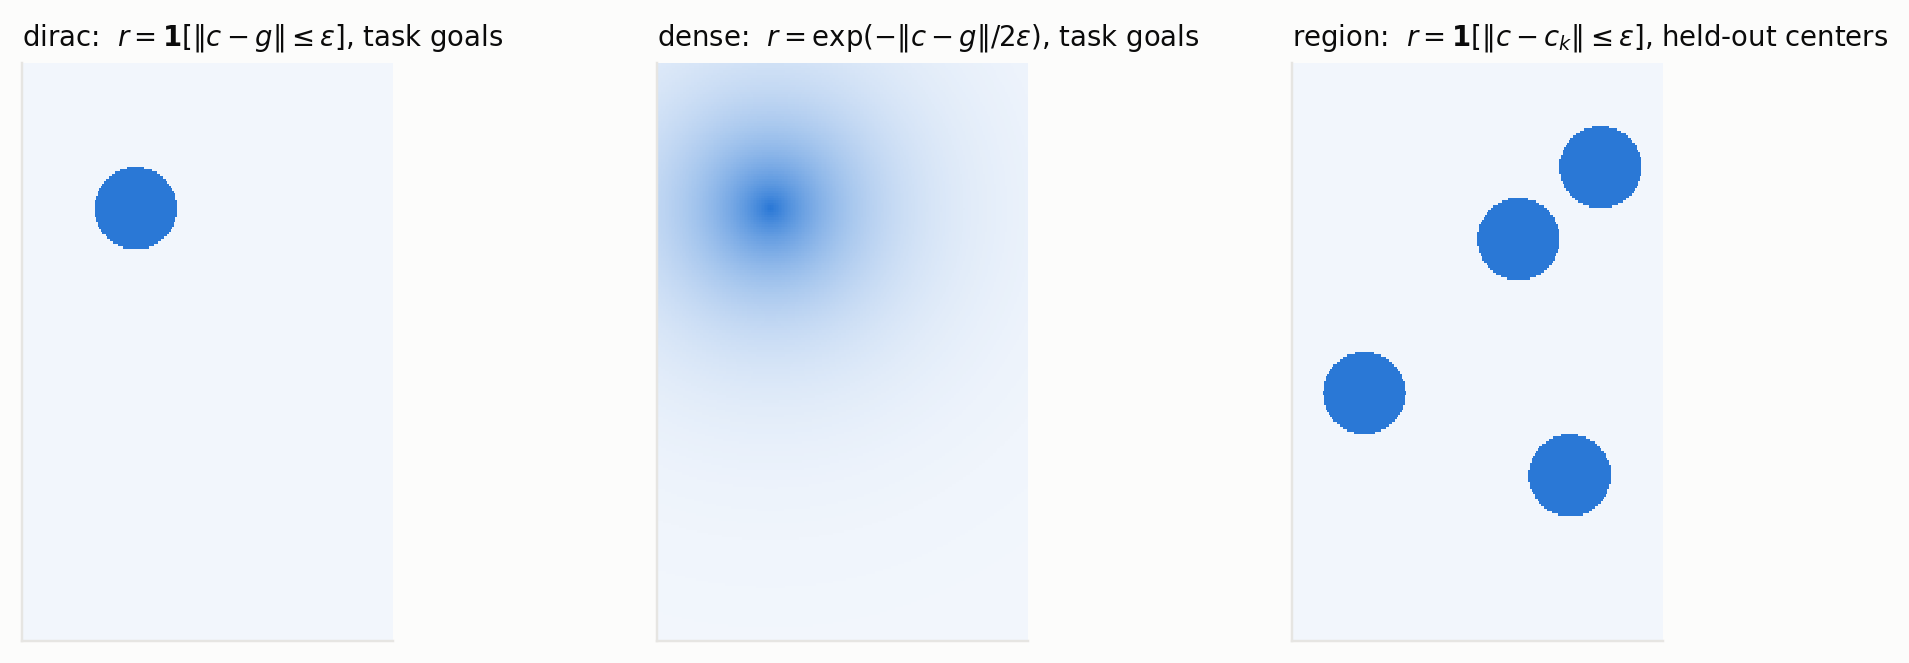
\includegraphics[width=0.95\textwidth]{figures/reward-families.png}
\caption{
The three test reward families on the cube workspace
(cube-position plane, $\epsilon$-balls to scale).
Sparse and dense share task-style centers and differ in shaping;
held-out regions keep the sparse form at hindsight-drawn dataset centers.
}
\label{fig:rewardfams}
\end{figure}

\begin{table}[h]
\centering
\small
\setlength{\tabcolsep}{4pt}
\begin{tabular}{llccc}
\toprule
Environment & Reward family & Plain FB & \DensityFB{} (soft) & \DensityFB{} (hard) \\
\midrule

\texttt{cube-single}
& sparse
& $0.413 \pm 0.308$
& $0.816 \pm 0.269$
& $\mathbf{0.888 \pm 0.091}$ \\

& dense
& $0.488 \pm 0.397$
& $0.725 \pm 0.301$
& $\mathbf{0.912 \pm 0.087}$ \\

& held-out regions
& $0.090 \pm 0.114$
& $0.293 \pm 0.052$
& $\mathbf{0.647 \pm 0.301}$ \\
\midrule

\texttt{cube-double}
& sparse
& $0.013 \pm 0.023$
& $0.549 \pm 0.240$
& $\mathbf{0.573 \pm 0.126}$ \\

& dense
& $0.037 \pm 0.011$
& $0.488 \pm 0.163$
& $\mathbf{0.520 \pm 0.121}$ \\

& held-out regions
& $0.000 \pm 0.000$
& $0.177 \pm 0.160$
& $0.167 \pm 0.014$ \\
\midrule

\texttt{scene}
& sparse
& $0.472 \pm 0.124$
& $0.395 \pm 0.092$
& $\mathbf{0.640 \pm 0.111}$ \\

& dense
& $0.413 \pm 0.030$
& $0.347 \pm 0.219$
& $\mathbf{0.627 \pm 0.094}$ \\

& held-out regions
& $0.053 \pm 0.080$
& $0.220 \pm 0.086$
& $\mathbf{0.347 \pm 0.038}$ \\
\bottomrule
\end{tabular}

\caption{
Zero-shot reward transfer
(mean $\pm$ $95\%$ CI, three seeds unless marked).
GCIQL has no reward readout of this kind and is therefore absent.
Plain FB is evaluated through its own reward interface, $z_r \propto \E_\rho[r(x)B(x)]$ followed by rollout under $z_r$, since it has no density readout; the reward families, pool, episode count, and success criterion are identical across all three columns, so only the readout differs.
All cells now use three seeds; the plain-FB seeds missing at first submission were trained to parity.
The plain-FB \texttt{cube-double} entries sit at the floor rather than merely low: they are $1$ and $0$ successes in $125$ episodes, against a random-index floor of $0.012$ and $0.000$.
All numbers use a $16{,}384$-configuration pool and $25$ episodes per task.
}
\label{tab:zeroshot}
\end{table}

\begin{table}[h]
\centering
\small
\begin{tabular}{lccc}
\toprule
\texttt{cube-single} ablation
& sparse
& dense
& held-out regions \\
\midrule

\DensityFB{} (soft)
& $0.816 \pm 0.269$
& $0.725 \pm 0.301$
& $0.293 \pm 0.052$ \\

Fixed partition ($K{=}256$)
& $0.725 \pm 0.121$
& $0.723 \pm 0.298$
& $0.133 \pm 0.201$ \\
\bottomrule
\end{tabular}
\caption{
Replacing the resampled query set with $256$ fixed prototypes at otherwise identical settings.
The largest drop occurs on held-out regions.
}
\label{tab:partition}
\end{table}

The largest difference appears on rewards centered away from the benchmark goals.
On \texttt{cube-single}, held-out-region transfer rises from $0.133$ with the fixed partition to $0.293$ with soft \DensityFB{} and $0.647$ with the hard variant (Table~\ref{tab:partition}).
This is consistent with continuous query representations helping most when the reward sits between or away from fixed prototypes.

Hard and soft targets behave differently across environments.
On \texttt{cube-single} and \texttt{scene}, the hard target improves all three reward families; on \texttt{scene}, for example, sparse transfer rises from $0.395$ to $0.640$.
On \texttt{cube-double}, however, the two targets sit inside each other's intervals ($0.549$ vs.\ $0.573$, $0.488$ vs.\ $0.520$, $0.177$ vs.\ $0.167$).
Hard targets therefore improve reward readout on some manipulation tasks and not others.
On goal reaching, the two variants are within noise everywhere (Table~\ref{tab:main}).

\paragraph{Comparison with published zero-shot methods.}
Table~\ref{tab:published} places our sparse-reward results alongside published state-based OGBench results from \citet{bagatella-iclr26a}.
This is not a controlled comparison.
The published results use $1$M gradient steps, $10$ seeds, and $10$ evaluation episodes per task, whereas ours use $500$k steps, three seeds, and $25$ episodes.
The task-index inference also differs: their methods use linear regression on relabeled data, whereas \DensityFB{} searches over candidate goals.
Our matched plain-FB column partially validates itself against that table: it reproduces the published FB result on \texttt{cube-single} ($0.536$ on the stock-hyperparameter seed, $0.413 \pm 0.308$ over the three seeds of Table~\ref{tab:zeroshot}, against $49.6$ published) and the \texttt{cube-double} floor (${\le}0.056$ vs $2.6$), but on \texttt{scene} our FB reaches ${\sim}0.45$ against a published $12.8$, so the published scene FB number should not be used as a comparison point for this stack; the matched local baseline is the honest one.
A related observation from the same probes: on \texttt{scene}, plain FB's reward interface outperforms its own goal conditioning ($0.45$ via $z_r$ vs $0.14$ native), so FB's weakness there is its goal encoding rather than its reward inference.

\begin{table}[h]
\centering
\small
\begin{tabular}{lccc}
\toprule
Method
& \texttt{cube-single}
& \texttt{cube-double}
& \texttt{scene} \\
\midrule

Laplacian \citep{wu2018laplacian}
& $15.1 \pm 1.5$
& $2.0 \pm 0.4$
& $7.8 \pm 1.3$ \\

RLDP \citep{jajoo-iclr26a}
& $19.8 \pm 2.4$
& $3.8 \pm 0.8$
& $11.6 \pm 1.6$ \\

ICVF \citep{ghosh2023reinforcement}
& $20.4 \pm 1.9$
& $5.0 \pm 0.8$
& $45.4 \pm 2.3$ \\

BYOL
& $22.0 \pm 3.2$
& $4.4 \pm 0.7$
& $15.4 \pm 1.4$ \\

TD-JEPA \citep{bagatella-iclr26a}
& $34.2 \pm 2.9$
& $3.6 \pm 0.8$
& $38.4 \pm 1.4$ \\

FB \citep{touati2021learning}
& $49.6 \pm 3.8$
& $2.6 \pm 0.4$
& $12.8 \pm 1.6$ \\

HILP \citep{park-iclr24a}
& $74.2 \pm 3.5$
& $20.0 \pm 2.7$
& $43.8 \pm 1.9$ \\

BYOL-$\gamma$
& $79.4 \pm 2.8$
& $2.6 \pm 0.7$
& $14.4 \pm 2.3$ \\
\midrule

\DensityFB{}
& $\mathbf{88.8 \pm 9.1}$
& $\mathbf{57.3 \pm 12.6}$
& $\mathbf{64.0 \pm 11.1}$ \\
\bottomrule
\end{tabular}

\caption{
Zero-shot success rate (\%) on state-based OGBench.
Rows above the line are as reported by \citet{bagatella-iclr26a} at $1$M gradient steps, $10$ seeds and $10$ episodes per task, with the task index inferred by linear regression.
Rows below are our sparse reward family at $500$k steps, three seeds and $25$ episodes, with the index chosen by search.
Our intervals are $t$-based on three seeds.
}
\label{tab:published}
\end{table}

The largest numerical gap is on \texttt{cube-double}: the strongest published result is $20.0$, while both \DensityFB{} variants exceed $54$.
On \texttt{scene}, hard \DensityFB{} reaches $64.0$ versus $45.4$ for the strongest published result.
The \texttt{cube-single} comparison is less informative: hard \DensityFB{} reaches $88.8$ versus $79.4$, but the difference lies within our three-seed confidence interval.
These comparisons remain suggestive until the protocols are matched.

\texttt{cube-double} is also where the published methods are closest to each other and to zero: six of the eight fall below $5$.

Reward transfer remains harder than direct goal reaching.
On \texttt{cube-double}, the same soft checkpoint reaches $0.736$ under ordinary goal conditioning and $0.549$ when the same task is specified through the sparse reward readout.
Because the checkpoint is identical, this gap enters through the reward-readout and goal-selection pipeline rather than through representation training.
An oracle that selects the reward center directly would separate readout error from goal-selection error.

% ======================================================================
\section{A latent task index}
\label{sec:latent}

Everything above conditions on a goal $g$.
Standard FB instead conditions on a latent vector $z$, which is what makes its zero-shot interface possible: any reward is embedded as $z_r \propto \E_\rho[r(x)B(x)]$ and executed by the policy indexed by $z_r$.
This section ports that interface to \DensityFB{}, shows where the direct port fails, and gives the correction.

\subsection{The direct port fails}
\label{sec:latent-fails}

The natural encoding replaces the goal with its backward embedding,
\begin{equation}
\label{eq:zenc}
z(g) = \sqrt d\;\frac{\bar B(\phi(g))}{\|\bar B(\phi(g))\|},
\end{equation}
trains the measure and actor on a mixture of hindsight indices $z(g)$ and random unit-sphere indices, and replaces the actor's kernel readout with the latent reward $r_z(u)=B(u)^\top z/\sqrt d$.
This collapses.
On \texttt{cube-double}, success falls from $0.736$ (goal-conditioned) to $0.017$, at the behavior-cloning floor of $0.019$; on \texttt{cube-single} the corresponding arms read $0.096$--$0.108$ against a floor of $0.111$.
The failure is not in the estimator: under $z$ the measure trains to the same cross-entropy as under $g$ and shows the same occupancy-ranking fidelity against Monte-Carlo rollouts.

\subsection{Diagnosis: the backward basis has an arbitrary, gauge-dominated geometry}

The cross-entropy loss constrains only the product $F^\top B$: for any invertible $C$, replacing $B$ by $CB$ and $F$ by $C^{-\top}F$ leaves every prediction unchanged.
The softmax adds a further exact invariance: for any constant vector $b$, replacing $B(x)$ by $B(x)+b$ shifts every logit in a row by the same $F^\top b$, which the softmax cancels.
The mean of $B$ is therefore pure gauge --- it can grow without changing a single predicted probability --- and training drives it to an extreme value.
Measured on every checkpoint, $\|\mu_B\|$ is $33$--$103$ times the average centered feature norm $\E\|B-\mu_B\|$, so the uncentered second moment $\Sigma_B=\E_\rho[B(x)B(x)^\top]$ is dominated by a single gauge direction: effective rank $1.0002$ of $d=50$, condition number $10^6$--$10^7$.
The centered covariance tells the opposite story: $\operatorname{Cov}(B)$ has effective rank $6.3$--$20.8$ of $50$ across the same checkpoints.
The informative geometry is rich; what looks like rank collapse is a softmax-gauge mean sitting on top of it.
Two consequences follow.

First, Equation~\ref{eq:zenc} collapses.
Normalizing $B(g)$ pins every goal to the gauge direction: over $4{,}096$ dataset goals, the mean pairwise cosine of $z(g)$ is $0.998$--$1.000$, where matched random unit vectors give $0.002$; subtracting the mean before normalizing drops it to ${\sim}0.003$.
The actor behaves accordingly: its output moves by $0.000$ when the goal index changes (noise floor $0.19$), while a random index moves it by $1.9$--$2.0$.
The policy is index-capable; the encoding never hands it two different indices.
The same collapse appears on goal-conditioned checkpoints that never trained with $z$, so it is a property of the encoding, not of latent training.

Second, FB's reward embedding is the wrong vector once the measure is normalized.
The identity behind $z_r\propto\E[rB]$ is linear --- $Q_r = F^\top \E[rB]$ holds because the FB value is linear in $B$ --- and the softmax removes exactly that linearity.
To read a reward through $r(u)\approx B(u)^\top c$, the correct coefficient is the least-squares one,
$c_r = (\Sigma_B+\lambda I)^{-1}\E[rB]$;
the moment $\E[rB]$ coincides with it only when $\Sigma_B\approx I$, which is what standard FB's orthonormality term enforces and \DensityFB{} deliberately removed.
With $\Sigma_B$ gauge-dominated, the two are nearly orthogonal: measured $\cos\!\left(\E[rB],\,c_r\right) = 0.010$--$0.025$.
The consequences are direct.
Reconstructing goal rewards as $B(u)^\top z$ scores AUC $0.43$--$0.87$ when $z$ is the moment or the point embedding of Equation~\ref{eq:zenc}, and $0.99$--$1.00$ when $z=c_r$.
Assigning rewards to their indices is at chance with the moment ($0.35$--$0.51$ coordinate percentile, where $0.50$ is chance) and matches the goal-indexed control with $c_r$ ($0.000$--$0.008$).
Consistent with the gauge diagnosis, centering alone recovers most of this: the centered point index $\operatorname{normalize}(B(g)-\mu_B)$ reconstructs rewards at AUC $0.99$--$1.00$ on the same pools (verified on disjoint fit and evaluation halves), while the inverse covariance additionally expands low-variance task directions and spreads the index set (participation ratio $28$--$30$ versus $6.6$--$19.8$ for centered pointing).

The uncentered encoder also fails an invariance a task code must have.
Adding a constant $\beta$ to a reward leaves its optimal policy unchanged but shifts the moment by $\beta\,\E[B]$ --- almost exactly the gauge direction --- and measured on our checkpoints the uncentered index of $r$ and of $r+1$ are nearly orthogonal ($\cos = 0.035$, $-0.000$, $-0.044$ on the three checkpoints tested), while the centered construction below is invariant to the digit.

\subsection{The corrected index}

The repair follows from the diagnosis: encode tasks with the least-squares coefficient rather than the moment, and let the actor integrate the actual reward rather than a latent surrogate.
Given a task specified by reward samples $\{(u_j, r_j)\}_{j=1}^M$,
\begin{equation}
\label{eq:dual-index}
\hat z = \sqrt d\, \frac{(\hat\Sigma_B+\lambda I)^{-1} \hat m}{\big\| (\hat\Sigma_B+\lambda I)^{-1} \hat m \big\|},
\qquad
\hat m = \frac1M \sum_{j} \bar B(u_j)\, r_j,
\end{equation}
where $\hat\Sigma_B$ is an exponential moving average of $\bar B(u)\bar B(u)^\top$ over query samples, stored with the network parameters so that training and evaluation whiten with the same statistics.
Hindsight goals supply reward samples for free through the kernel of Equation~\ref{eq:goal-readout}, $r_j = k_j^\epsilon(g)$.
The measure and the actor condition on $\hat z$; the actor's scalar critic integrates the reward samples themselves,
\begin{equation}
q_{\hat z}(s,a) = \sum_j p_j(s,a,\hat z)\, r(u_j),
\end{equation}
so the latent serves only as a policy index and the reward semantics stay external --- the same division of labor that makes the goal-conditioned readout work.
This is whitening at the interface rather than in the loss: the orthonormality penalty that would make $\E[rB]$ correct also caps manipulation success at $0.225$ (Section~\ref{sec:todo}), so the basis is left free and the correction is applied where the index is built.

The gauge analysis identifies one further correction, which the first corrected-index run predates and the centered arms of Section~\ref{sec:latent} implement.
Because the mean of $B$ is unidentifiable and reward shifts move the moment along it, the principled statistics are the centered ones:
\begin{equation}
\label{eq:centered-index}
\hat z^{\,\mathrm{c}} = \sqrt d\, \frac{(\hat C_B+\lambda I)^{-1} \hat m^{\mathrm{c}}}{\big\| (\hat C_B+\lambda I)^{-1} \hat m^{\mathrm{c}} \big\|},
\qquad
\hat m^{\mathrm{c}} = \frac1M \sum_j \left(\bar B(u_j)-\hat\mu_B\right)\left(r_j - \bar r\right),
\end{equation}
with $\hat\mu_B$ and $\hat C_B$ the running mean and centered covariance and $\bar r$ the sample-mean reward.

\begin{proposition}[Invariances of the centered index]
\label{prop:invariance}
$\hat z^{\,\mathrm{c}}$ is invariant to the gauge translation $B(x)\mapsto B(x)+b$, to the reward shift $r\mapsto r+\beta$, and, after normalization, to positive reward scaling $r\mapsto\alpha r$.
The uncentered index of Equation~\ref{eq:dual-index} has only the last of these.
\end{proposition}
\emph{Proof sketch.} Centering removes both translations exactly: $(B+b)-(\mu_B+b)=B-\mu_B$ and $(r+\beta)-(\bar r+\beta)=r-\bar r$, and $\hat C_B$ is unchanged by either; scaling $r$ by $\alpha>0$ scales $\hat m^{\mathrm{c}}$ linearly and is absorbed by the normalization. \hfill$\square$

Two scope notes on this proposition.
First, it corrects the \emph{additive} gauge only: the factorization also admits $B\mapsto AB$, $F\mapsto A^{-\top}F$ for invertible $A$, under which the coefficient transforms dually ($c\mapsto A^{-\top}c$ at $\lambda=0$) but isotropic ridge regularization and sphere normalization are not invariant, so the encoder is translation-gauge-invariant, not fully gauge-invariant.
The additive direction is the empirically dominant pathology.
Second, the invariance is exact for the population object; the implementation tracks $\hat\mu_B$ and $\hat C_B$ as moving averages during joint training, and only approximates it (both moments run on the same schedule against the same base measure --- the batch next-state marginal used for queries --- with $\hat C_B$ symmetrized and eigenvalue-floored, and the mismatch between stored and probe statistics logged).

The centered encoder also forces an interface split that the uncentered form obscured.
Its reward-sample moment vanishes identically at $M=1$ ($r_1-\bar r=0$), so it has no one-sample limit: point-goal prompting and reward-sample prompting are different inference modes.
For goals we use the \emph{analytic centered point prompt} $z_g = \sqrt d\,\operatorname{normalize}(\bar B(\phi(g))-\hat\mu_B)$ --- the population moment of a Dirac-style goal reward --- while the general interface consumes an actual sample set with $M>1$ (in practice $M\ge256$), and results for one mode are not evidence for the other.
A constant reward has $\hat m^{\mathrm{c}}=0$ exactly; the implementation returns a neutral index when $\|(\hat C_B+\lambda I)^{-1}\hat m^{\mathrm{c}}\|$ falls below a threshold, since normalizing a near-zero coefficient would amplify noise.

\subsection{Result}

Both links of the repair were verified on existing checkpoints before retraining: the ridge solve de-collapses the index (participation ratio $1.0\to 9$--$38$), and the least-squares coefficient fixes reward reconstruction and assignment as quoted above.
We then retrained with the corrected index (\texttt{cube-single}, $500$k steps, one seed per arm), in both encodings and in both inference modes that the centering forces apart (see the discussion after Proposition~\ref{prop:invariance}).
The \emph{analytic point prompt} encodes a goal as the population moment of a Dirac-style goal reward, $\hat z \propto (\hat\Sigma_B+\lambda I)^{-1}\bar B(\phi(g))$; the \emph{reward-sample} prompt is the general interface, and builds $\hat z$ from an actual set of $M=256$ samples $\{(u_j,r_j)\}$ drawn from a frozen pool, with no one-sample shortcut available to it.
Evaluation is noisy at this budget, so we report the $500$k value and the mean over evaluations after $350$k:

\begin{center}
\small
\setlength{\tabcolsep}{4pt}
\begin{tabular}{llcc}
\toprule
Index & Prompt at evaluation & at $500$k & mean $\ge 350$k \\
\midrule
centered, Eq.~\ref{eq:centered-index} & reward samples, $M{=}256$ & $\mathbf{0.816}$ & $0.785$ \\
centered, Eq.~\ref{eq:centered-index} & analytic point & $0.824$ & $0.868$ \\
uncentered, Eq.~\ref{eq:dual-index} & analytic point & $0.812$ & $0.743$ \\
uncentered, actor uses $B^\top \hat z$ & analytic point & $0.368$ & $0.291$ \\
\midrule
uncorrected latent arms & --- & $0.096$--$0.108$ & --- \\
behavior cloning & --- & $0.111$ & --- \\
goal-conditioned \DensityFB{} (soft) & goal & $0.929$ & --- \\
\bottomrule
\end{tabular}
\end{center}

The corrected index with the sample-based readout is the first latent-conditioned \DensityFB{} that works: roughly $7.5\times$ the uncorrected arms and $88\%$ of the goal-conditioned anchor.
Three readings follow from the rows.
First, the top row is the general interface actually exercised: that number comes from a rollout whose index was built from $256$ reward samples, not from the point shortcut, and it matches the point prompt on the same encoder ($0.816$ against $0.824$), so for goal-kernel rewards the two inference modes agree.
Second, centering costs nothing: the centered arms reach $0.824$ and $0.816$ against $0.812$ for the uncentered encoder, so the invariances of Proposition~\ref{prop:invariance} are bought for free, and we take the centered index of Equation~\ref{eq:centered-index} as the method and keep the uncentered run as an ablation.
Third, the gap between the last two rows isolates the readout: conditioning is identical, so integrating real reward samples versus the linear surrogate $B^\top\hat z$ accounts for $0.812$ versus $0.368$.
During training the index stays de-collapsed, and on the uncentered run the actor's index sensitivity rises from exactly $0.000$ to $0.132$ (measured at $100$k steps), with the earlier pathology inverted: goal-derived indices now move the policy more than random ones ($0.132$ vs $0.065$).
